%%%%%%%%%%%%%%%%%%%%%%%%%%%%%%%%%%%%%%%%%%%%%%%%%%%%%%%%%%%%%%%%
\section{Multi-Model Component}
\label{sec:impl_multi_model}

Runtime model switching allows one physical subsystem to use different internal models in different operating regimes.
The implementation realizes \ref{req:UR-09} and the derived requirements \ref{req:SR-09-01}--\ref{req:SR-09-04}.
The \texttt{MultiComponent} class implements this behavior as a component wrapper with a fixed external interface and one active internal model.
Section~\ref{sec:architecture_multicomponent} introduces the architectural roles of wrapper, mode selector, hysteresis, and state adapter.
The following subsections describe how \texttt{MultiComponent} realizes these roles.

%%%%%%%%%%%%%%%%%%%%%%%%%%%%%%%%%%%%%%%%%%%%%%%%%%%%%%
\subsection{Scope and Component Contract}
\label{sec:impl_multi_model_scope}

The \texttt{MultiComponent} class extends \texttt{CoSimComponent} with a registry of interchangeable internal models.
Each registered model is itself a \texttt{CoSimComponent}.
The surrounding \texttt{System} interacts only with the wrapper component.
It does not depend on the currently active internal model.

At runtime, exactly one model is active.
The wrapper identifies it through \texttt{active\_mode} and accesses it through \texttt{active\_comp}.
The active model performs the time step, provides the wrapper outputs, and serves as the source for state access and hybrid hooks.
Input assignment is handled separately, because incoming inputs are forwarded to the active model and cached for a possible later switch.
A user-defined \texttt{mode\_selector} may request a different mode before a step is executed.
On an accepted switch, the wrapper transfers the physical state from the current model to the target model.

Subclasses provide the model-specific parts of this process.
They register the available models and define how state is adapted between model interfaces.
Table~\ref{tab:multi_component_contract} summarizes the main contract.

\begin{table}[t]
  \centering
  \caption[Multi-component extension points.]{Main extension points and state fields of \texttt{MultiComponent}.}
  \label{tab:multi_component_contract}
  \begin{tabular}{lp{9.5cm}}
    \toprule
    \textbf{Element}                  & \textbf{Role}                                                                                                   \\
    \midrule
    \texttt{models}                   & Implements the model registry by storing available model implementations by mode key                            \\
    \addlinespace
    \texttt{active\_mode}             & Stores the key of the currently active model selected by the mode-switching wrapper                             \\
    \addlinespace
    \texttt{active\_comp}             & References the active component instance to which lifecycle and stepping calls are delegated                    \\
    \addlinespace
    \texttt{mode\_selector}           & Implements the mode selector by deriving the requested mode from the current time and selector-specific context \\
    \addlinespace
    \texttt{hysteresis}               & Implements the hysteresis support by blocking rapid switching when a dwell time is configured                   \\
    \addlinespace
    \texttt{\_allow\_mode\_switching} & Guards mode selection during trial steps and algebraic output evaluation                                        \\
    \addlinespace
    \texttt{\_adapt\_state()}         & Implements the state adapter by mapping the exported state to the target model interface                        \\
    \addlinespace
    \texttt{\_latest\_inputs}         & Caches the most recent external inputs so they can be replayed on the target model during a switch              \\
    \addlinespace
    \texttt{sync\_events}             & Records performed switches for inspection and debugging                                                         \\
    \addlinespace
    \bottomrule
  \end{tabular}
\end{table}

%%%%%%%%%%%%%%%%%%%%%%%%%%%%%%%%%%%%%%%%%%%%%%%%%%%%%%
\subsection{Initialization and Interface Unification}
\label{sec:impl_multi_model_initialization}

A concrete subclass registers its internal models during construction.
It stores them in \texttt{models}, selects the initial model through \texttt{active\_mode}, and stores the corresponding component in \texttt{active\_comp}.
The subclass then calls \texttt{\_unify\_ports()} before the wrapper is registered with a \texttt{System}.
This construction-time setup is required because signal connections are validated before component initialization.

The wrapper must expose one stable port interface to the surrounding system.
For this purpose, \texttt{\_unify\_ports()} adopts the input and output specifications of the active component.
It then checks that every registered model provides compatible ports with the same names, directions, port types, and units.
If a model misses a required port or exposes an incompatible specification, construction fails with a \texttt{ValueError}.
This ensures that a later mode switch cannot change the external interface of the component.

Direct-feedthrough metadata must also remain fixed.
The wrapper compares the feedthrough dictionaries of all registered models during initialization.
A mismatch is rejected.
Section~\ref{sec:impl_structural} assumes fixed zero-delay behavior for every component during a simulation run.
The \texttt{MultiComponent} class can therefore switch models only when the externally visible dependency structure remains unchanged.

%%%%%%%%%%%%%%%%%%%%%%%%%%%%%%%%%%%%%%%%%%%%%%%%%%%%%%
\subsection{Runtime Model Switching}
\label{sec:impl_multi_model_switching}

Runtime switching is part of the component step.
When a master algorithm calls \texttt{do\_step(t, dt)} on the wrapper, the base component logic delegates to \texttt{\_do\_step\_internal(t, dt)}.
Zero-duration calls are treated as output-refresh evaluations.
They are delegated to the current active model without mode selection.
For positive step sizes, the wrapper first checks the switching guards.
Mode selection is skipped when switching is disabled, when no selector is configured, or when the hysteresis dwell window is active.
The selector is evaluated only after these guards pass.
Figure~\ref{fig:impl_multi_model_switching} summarizes the switching path.

\begin{figure}[t]
  \centering
  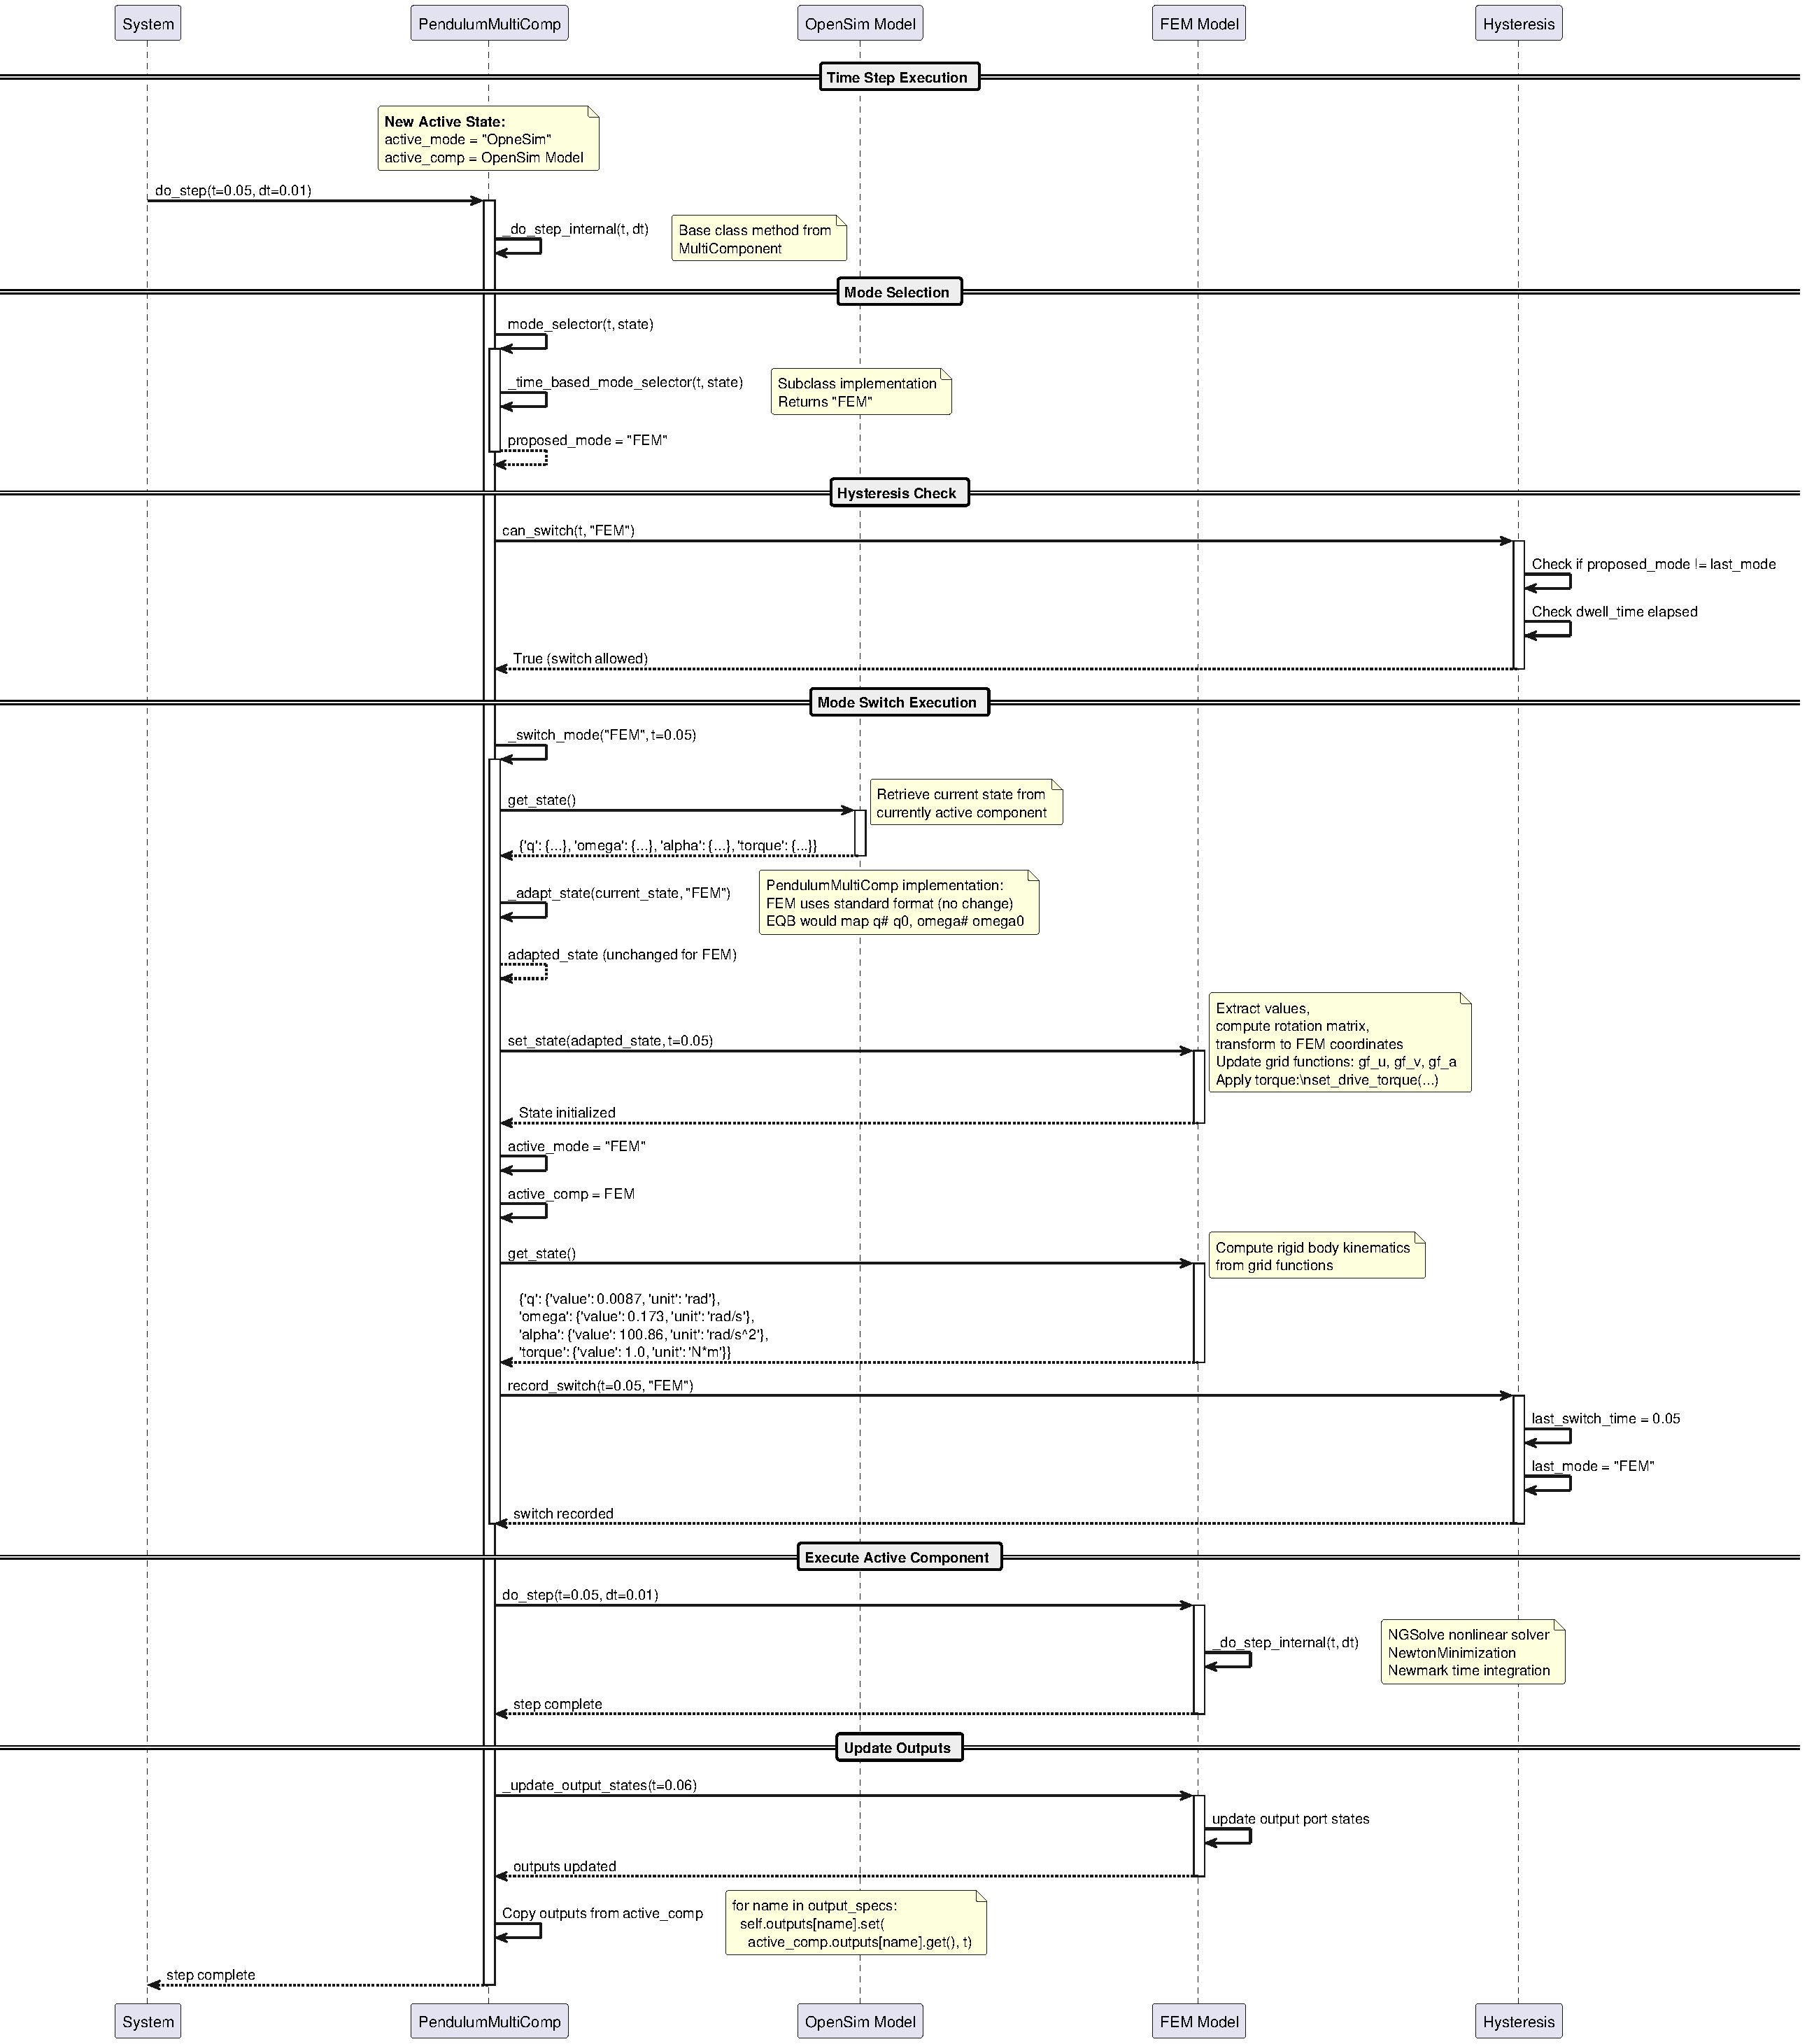
\includegraphics[width=\textwidth]{diagrams/out/pdf/execution/MultiComponent_Switching.pdf}
  \caption[Runtime switching sequence.]{Runtime switching sequence of the \texttt{MultiComponent} class for a positive macro step.
  The wrapper applies switching guards, transfers state and cached inputs on an accepted switch, and delegates the step to the active model.}
  \label{fig:impl_multi_model_switching}
\end{figure}

A configured \texttt{Hysteresis} object may block a requested switch.
During the dwell window, the wrapper keeps the current mode and does not call the selector.
Outside the dwell window, the selector returns the requested mode.
If the requested mode equals the current mode, the wrapper keeps the current model for this step.
This prevents rapid switching near decision boundaries.

If the requested mode is accepted, \texttt{\_switch\_mode()} performs the transition.
It first retrieves the current state from the active model.
The state is then passed to \texttt{\_adapt\_state()}.
This hook maps the state to the format expected by the target model.
The adapted state is written to the target component through \texttt{set\_state()}.
The wrapper then updates \texttt{active\_mode} and \texttt{active\_comp}.

Each accepted switch is stored in \texttt{sync\_events}.
The stored entry contains the switch time and the two involved modes.
Detailed source and target state snapshots are recorded only when \texttt{record\_switch\_state} is enabled.
This log is used to inspect whether the state transfer behaved as expected.

After the optional mode switch, the actual time step is delegated to the active component through \texttt{do\_step(t, dt)}.
The master algorithm therefore does not need a special execution path for multi-model components.
The internal mode selection remains encapsulated inside the wrapper.
Section~\ref{sec:impl_multi_model_state_events} describes how input forwarding, output propagation, and hybrid delegation are handled around the active model.

%%%%%%%%%%%%%%%%%%%%%%%%%%%%%%%%%%%%%%%%%%%%%%%%%%%%%%
\subsection{Input, Output, and Hybrid Delegation}
\label{sec:impl_multi_model_state_events}

The \texttt{set\_inputs()} method forwards incoming values to the active model and stores them in \texttt{\_latest\_inputs}.
Inactive models are not advanced and do not receive every input update.
During an accepted switch, the cached inputs are replayed on the target model before the adapted state is written.
The target model is therefore synchronized with the most recent external inputs at the switch time.

Output propagation follows the opposite direction.
After the active model has advanced, \texttt{\_update\_output\_states()} copies the active model outputs to the wrapper ports.
The surrounding \texttt{System} therefore reads outputs only from the \texttt{MultiComponent}.
Event ports are handled in the same update step.
Ports corresponding to triggered events are set to \texttt{True}, while inactive event ports are reset to \texttt{False}.

Algebraic output evaluation uses the same active-model delegation.
The wrapper temporarily disables runtime model switching during \pyfn{evaluate\_outputs()}.
It evaluates the active model for the supplied trial inputs.
The resulting values are copied to the wrapper ports.
This prevents direct-feedthrough detection from changing the active model.
It also prevents \ac{IJCSA} residual evaluations from changing the active model.

State access is routed through the active model.
The \texttt{get\_state()} method returns the state of \texttt{active\_comp}.
The \texttt{set\_state()} method adapts the provided state to the active mode and writes it to \texttt{active\_comp}.
The wrapper therefore provides one access point.
The concrete state schema remains defined by the active model and the subclass adaptation logic.

The hybrid hooks are delegated to the active model as well.
Event indicator evaluation, crossing detection, rollback snapshots, event handling, and internal event hints are forwarded to \texttt{active\_comp}.
Runtime model switching can be disabled through \texttt{\_allow\_mode\_switching}.
The hybrid algorithm uses this flag during trial steps.
Event detection and localization therefore cannot change the active model while a rollback snapshot is valid.

%%%%%%%%%%%%%%%%%%%%%%%%%%%%%%%%%%%%%%%%%%%%%%%%%%%%%%
\subsection{Verification}
\label{sec:impl_multi_model_verification}

The verification scenario isolates the switching mechanism through a two-mode integrator with a known analytical reference.
The wrapper holds two scalar integrators that share the input and output interface but apply different gains to the constant input $u = 1$.
Mode~A integrates with $k_A = 1.0$ and Mode~B with $k_B = 2.0$.
Both models share the state variable $x$ with $x(0) = 0$.
A \texttt{mode\_selector} switches from Mode~A to Mode~B at the analytical time $t_s = 0.5\,$s.

The expected trajectory is piecewise linear with slope $k_A$ before the switch and slope $k_B$ after.
The state must remain continuous at $t_s$, since \texttt{\_switch\_mode()} adapts and transfers the active state to the target model before the next time step.

Figure~\ref{fig:impl_multi_model_verification} compares the numerical trajectory with the analytical reference and shows the active mode over time.

\begin{figure}[!htbp]
  \centering
  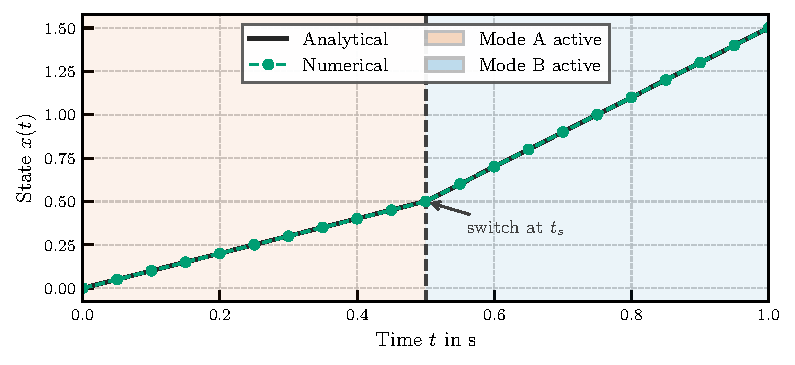
\includegraphics[width=0.82\linewidth]{figures/5_implementation/multi_component/multi_component_switching_verification.pdf}
  \caption[Two-model integrator check for runtime model switching]{Two-model integrator check for runtime model switching.
    The trajectory follows the analytical reference and remains continuous at the accepted switch time.}
  \label{fig:impl_multi_model_verification}
\end{figure}

The numerical trajectory matches the analytical solution within machine precision.
The maximum absolute error is $3.3\cdot 10^{-16}$.
The active mode changes from A to B exactly at $t_s$.
The recorded \texttt{sync\_events} entry confirms one accepted switch with retrieved and synchronized states equal to $x(t_s)=0.5$.
The hysteresis path is covered by the unit tests and is not repeated here.